\section{提案手法}
\begin{itemize}
  \item 前項の内容から、前処理は行わず、固定の画素値にとらわれずに異常胃を判別する方法を考える。
  \begin{itemize}
    \item[→] まず、健常胃の特徴は、画像を識別できるほどの特徴ではないと考え、
    異常胃のマスクメロン模様で判別しようと考えた。
    マスクメロン模様は異常胃の全ての画像に、びっしりと敷き詰められている。
    これを、異常胃には同じようなパーツが複数存在していると見立たてると、
    同じようなパーツが複数存在したら、異常胃であり、そうでなければ健常胃であると判別できると考えた。
    \begin{itemize}
      \item[→] そこで、私は3×3の配列を作成し、ある画素の周りを含めた9画素をその配列に格納し、中心の画素値と周りの
      8画素を比較する方法を考えた。この方法では具体的な画素値は必要とせず、比較を行うだけであるため、それぞれ画素値が違うマスクメロン模様の特徴を
      とらえることができると考えた。そのため、これを全画素に対して行い、比較の結果の合計を特徴量として、距離を計算し、ソートすることで異常胃を判別
      できると考えた。
    \end{itemize}
  \end{itemize}
\end{itemize}
以下に具体的な手順を示す。

\begin{enumerate}
  \item 図\ref{graph:1}のように、全画像の読み込みを行い、図\ref{graph:2}のインスタンスを作成。
  \item 画素値を入れるための3×3の配列を作成する。
  \item ある座標(x,y)の画素値と周りの座標(y-1,x-1)~(y+1,y+1)の画素値を配列に格納する。
  \item 図\ref{graph:3}のようにして、図\ref{graph:4}のような評価関数を呼び出し、中心の画素値と周りの画素値を比較する。
  \item (y-1,x-1)~(y+1,y+1)まで行い、中心の画素値より大きければ、配列pm[0]~pm[7]の値を1増やして、小さければ、配列pm[8]~pm[15]の値を1増やす。
  \item 上記の処理を端1画素を除いた全画素に行うまでループする。
  \item 配列pm[0]~pm[15]の値をその画像の特徴量として扱い、それぞれの画像と入力画像の特徴量の距離を図\ref{graph:5}のように求める。
  \item 距離が近い順に判別結果とする。
\end{enumerate}

\begin{figure}[htbp]
  \begin{minipage}[t]{0.45\hsize}
    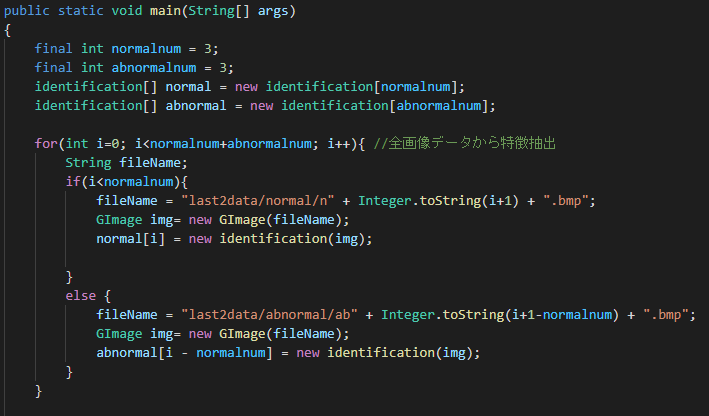
\includegraphics[scale=0.4]{画像読み込み.PNG}
    \centering
    \caption{画像読み込み}
    \label{graph:1}
  \end{minipage}
  \begin{minipage}[t]{0.25\hsize}
    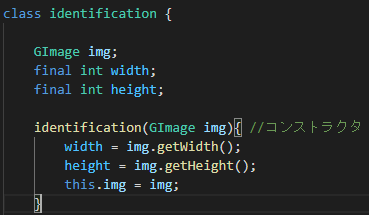
\includegraphics[scale=0.4]{クラス.PNG}
    \centering
    \caption{idenficationクラス}
    \label{graph:2}
  \end{minipage}
  \begin{minipage}[t]{0.25\hsize}
    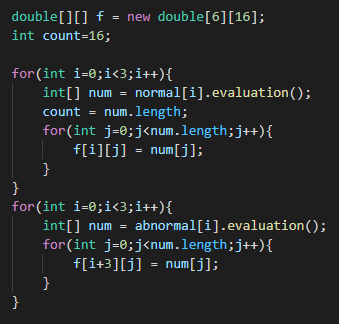
\includegraphics[scale=0.4]{評価関数呼び出し.PNG}
    \centering
    \caption{評価関数呼び出し}
    \label{graph:3}
  \end{minipage}
  \begin{minipage}[t]{0.45\hsize}
    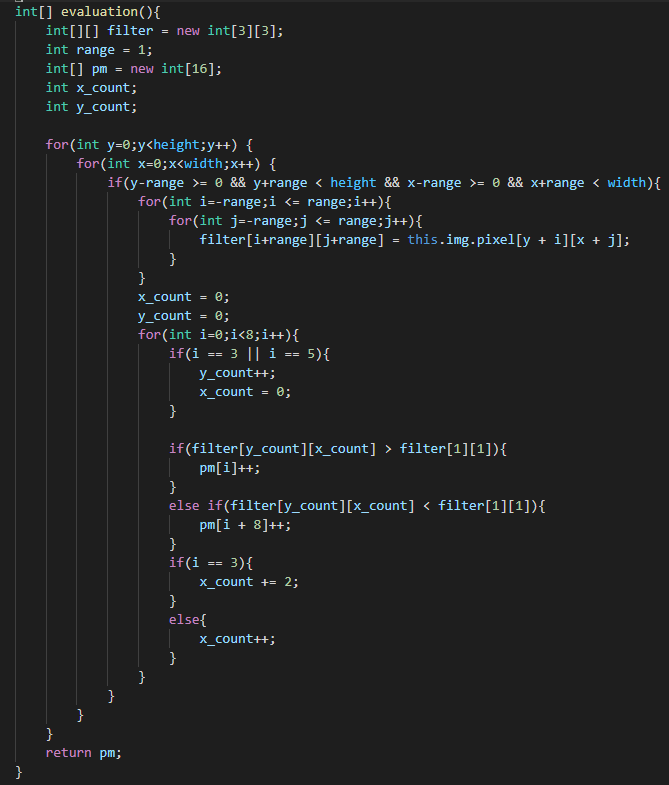
\includegraphics[scale=0.4]{評価関数.PNG}
    \centering
    \caption{評価関数}
    \label{graph:4}
  \end{minipage}
  \begin{minipage}[t]{0.45\hsize}
    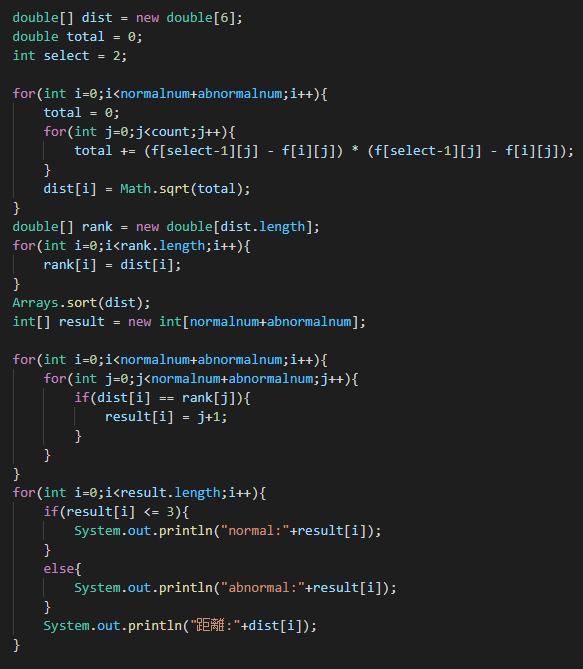
\includegraphics[scale=0.4]{距離計算.PNG}
    \centering
    \caption{距離計算とソート}
    \label{graph:5}
  \end{minipage}
\end{figure}
